\documentclass[tikz,convert={outfile=\jobname.svg}]{standalone}
\usetikzlibrary{arrows, shapes}
\usepackage{amsmath}

\begin{document}

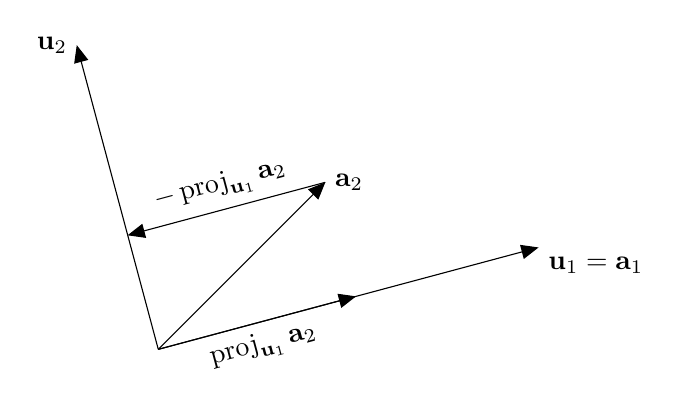
\begin{tikzpicture}
  \draw [-triangle 45] (0, 0) -- (15:5) node [below right] {$\mathbf{u}_1 = \mathbf{a}_1$};
  \draw [-triangle 45] (0, 0) -- (105:4) node [left] {$\mathbf{u}_2$};
  \draw [-triangle 45] (0, 0) -- (15:2.6) node [pos=0.5, below, rotate=15] {$\operatorname{proj}_{\mathbf{u}_1} \mathbf{a}_2$};
  \draw [-triangle 45] (0, 0) -- (45:3) node [right] {$\mathbf{a}_2$};
  \draw [-triangle 45] (45:3) -- ++(195:2.6) node [pos=0.5, above, rotate=15] {$-\operatorname{proj}_{\mathbf{u}_1} \mathbf{a}_2$};
\end{tikzpicture}
     
\end{document}


